\chapter{Entanglement, Density Matrices, and Locality}

This lecture begins by postponing Bell's theorem as a theorem and asking instead what entanglement is really telling us. The first correction is already important: the issue is not that two systems somehow ``share a state.'' A composite system always has a state. The real question is whether that state is a product state. To make that sharp, we first need wave functions as coordinates in Hilbert space; then we can see what factorization means, why the singlet state defeats it, why a reduced density matrix is the right local description of one part of an entangled pair, and finally why none of this allows signals to outrun light even though it does force us to think more carefully about locality.

\section{Wave Functions As Coordinates In Hilbert Space}

Susskind pauses early to clean up the language. Entanglement is not a mystical sharing of a state. The composite system has a state whether it is entangled or not. What distinguishes entanglement is that the state of the composite system need not factor into a state of Alice's subsystem times a state of Bob's subsystem.

That is easiest to say once a state has been written in components. So let us begin with the notion of a wave function. A wave function may or may not have anything to do with waves. Historically the word came from examples in which particles were described by wave-like probability amplitudes, but logically the construction is much more general. One starts with a state vector
\[
|\Psi\rangle
\]
and a basis of vectors labeled by a complete set of commuting observables. We shall denote those labels by
\[
a,b,c,\ldots
\]
with the understanding that a single system may require one label or many.

\begin{figure}[ht]
\centering

\includegraphics[width=0.72\textwidth]{lecture_07_figure_02.png}
\end{figure}

The board at this point is partly obscured, but the intent is clear: first the abstract expansion of the state vector, and then the identification of the coefficients with the wave function. In clean notation we write
\begin{equation}
\psi(a,b,c,\ldots)=\langle a,b,c,\ldots|\Psi\rangle
\end{equation}
and therefore
\begin{equation}
|\Psi\rangle=\sum_{a,b,c,\ldots}\psi(a,b,c,\ldots)\,|a,b,c,\ldots\rangle.
\end{equation}
The wave function is thus the set of coefficients used to expand the vector in the chosen basis, or equivalently the set of inner products of the state with the basis vectors.

For a single spin there is only one label if we choose, say, the $\sigma_z$ basis: the label takes the values $\uparrow$ and $\downarrow$. For two spins there are two labels, one for each subsystem. For a particle in three-dimensional space, one may use three commuting coordinates. The wave function is not a special object attached only to particles in space; it is simply the coordinate description of a vector once a basis has been chosen.

There is a useful side remark here. If one changes basis, for example from the $\sigma_z$ basis to the $\sigma_x$ basis, the wave function changes. In that sense, changing basis plays the role that a Fourier transform plays in familiar examples. The state vector itself is the same; what changes is the coordinate description of that vector.

\section{Expectation Values And Composite Systems}

Once the wave function is in hand, expectation values become explicit calculations. Let $L$ be an observable. Its matrix elements in the chosen basis are
\begin{equation}
L_{a'a}=\langle a'|L|a\rangle.
\end{equation}
If
\[
|\Psi\rangle=\sum_a \psi(a)\,|a\rangle,
\qquad
\langle\Psi|=\sum_{a'} \psi^*(a')\,\langle a'|,
\]
then the expectation value of $L$ is
\begin{align}
\langle L\rangle
&=\langle\Psi|L|\Psi\rangle \\
&=\sum_{a',a}\psi^*(a')\,\langle a'|L|a\rangle\,\psi(a) \\
&=\sum_{a',a}\psi^*(a')\,L_{a'a}\,\psi(a).
\end{align}
This is the basic machine. Every expectation value is computed from a wave function, its complex conjugate, and the matrix elements of the observable.

Now we pass to a composite system. Let $a$ label Alice's basis states and $b$ label Bob's. The lecture emphasizes that the pair $(a,b)$ should be thought of as a single label for a basis vector of the combined Hilbert space.

\begin{figure}[ht]
\centering

\includegraphics[width=0.56\textwidth]{lecture_07_figure_03.png}
\end{figure}

The notation ladder on the board is pedagogical: one first sees subsystem kets, then the composite ket, then the generic state. In clean form,
\begin{align}
|a\rangle \\
|b\rangle \\
|a,b\rangle \\
|\Psi\rangle
\end{align}
where $|a,b\rangle$ is one basis vector of the tensor-product space.

The composite wave function is then
\begin{equation}
\Psi(a,b)=\langle a,b|\Psi\rangle.
\end{equation}
The state itself may be expanded as
\begin{equation}
|\Psi\rangle=\sum_{a,b}\Psi(a,b)\,|a,b\rangle.
\end{equation}

What about observables? Suppose $L$ is an observable belonging to Alice and $M$ is an observable belonging to Bob. In the combined Hilbert space, Alice's observable acts on Alice's factor and does nothing to Bob's. Therefore its matrix elements are
\begin{equation}
L_{a'b';ab}=L_{a'a}\,\delta_{b'b}.
\end{equation}
Likewise Bob's observable acts trivially on Alice's factor:
\begin{equation}
M_{a'b';ab}=\delta_{a'a}\,M_{b'b}.
\end{equation}
That innocent-looking Kronecker delta is the whole idea. Alice's operator is the same operator she would have written if Bob did not exist, tensored with the identity on Bob's Hilbert space.

\section{Product States, Correlations, And The First Test For Entanglement}

We can now say exactly what a product state is.

\begin{definition}
A composite state is a product state if its wave function factorizes:
\begin{equation}
\Psi(a,b)=\psi_A(a)\,\phi_B(b).
\end{equation}
\end{definition}

This is not a decorative algebraic property. It means precisely that Alice has a wave function of her own and Bob has a wave function of his own, with no additional joint structure.

Let us check the expectation value of an Alice observable in such a state. By the general rule,
\begin{align}
\langle L_A\rangle
&=\sum_{a',a,b',b}\Psi^*(a',b')\,L_{a'b';ab}\,\Psi(a,b) \\
&=\sum_{a',a,b',b}\psi_A^*(a')\phi_B^*(b')\,L_{a'a}\delta_{b'b}\,\psi_A(a)\phi_B(b).
\end{align}
The Kronecker delta sets $b'=b$, so
\begin{align}
\langle L_A\rangle
&=\sum_{a',a,b}\psi_A^*(a')\,L_{a'a}\,\psi_A(a)\,\phi_B^*(b)\phi_B(b) \\
&=\left(\sum_{a',a}\psi_A^*(a')\,L_{a'a}\,\psi_A(a)\right)
\left(\sum_b \phi_B^*(b)\phi_B(b)\right).
\end{align}
If Bob's state is normalized, the second factor is $1$, and therefore
\begin{equation}
\langle L_A\rangle=\sum_{a',a}\psi_A^*(a')\,L_{a'a}\,\psi_A(a).
\end{equation}
That is exactly the formula Alice would have written if Bob were absent. In a product state, Alice's local statistics are just Alice's.

The same argument works for Bob. More interesting is the expectation value of a product operator $L_A M_B$. In a product state one finds
\begin{align}
\langle L_A M_B\rangle
&=\sum_{a',a,b',b}
\psi_A^*(a')\phi_B^*(b')\,L_{a'a}M_{b'b}\,\psi_A(a)\phi_B(b) \\
&=\left(\sum_{a',a}\psi_A^*(a')L_{a'a}\psi_A(a)\right)
\left(\sum_{b',b}\phi_B^*(b')M_{b'b}\phi_B(b)\right) \\
&=\langle L_A\rangle\,\langle M_B\rangle.
\end{align}
Thus the product of expectation values and the expectation value of the product agree for product states.

This immediately suggests the first operational test for entanglement. Define the correlation
\begin{equation}
C(L,M)=\langle LM\rangle-\langle L\rangle\langle M\rangle.
\end{equation}
If one can find any Alice observable $L$ and any Bob observable $M$ for which $C(L,M)\neq 0$, then the state cannot be a product state. It is entangled.

\subsection{Question \& Answer}

What does $LM$ mean here? It does \emph{not} mean ``measure $M$ and then measure $L$.'' The lecture pauses over this because the notation invites the wrong interpretation. $LM$ is the operator product: first $M$ acts on the vector, then $L$ acts on the result. That is a mathematical operation in Hilbert space, not the physical act of measurement. In the present case the distinction is especially clean because $L$ acts on Alice's subsystem and $M$ acts on Bob's, so the two operators commute:
\begin{equation}
[L,M]=0.
\end{equation}
Their order does not matter, but that still does not turn the symbol $LM$ into a sequence of laboratory measurements.

\section{The Singlet State And Knowing The Whole But Not The Parts}

The singlet state is the lecture's sharp counterexample to product structure. We keep Susskind's slot order: the first entry refers to Bob, the second to Alice. The state is
\begin{equation}
|\Psi_{\mathrm{sing}}\rangle
=
\frac{1}{\sqrt2}
\left(
|\uparrow\downarrow\rangle
-
|\downarrow\uparrow\rangle
\right).
\end{equation}
This is not a product state.

Let us begin with the simplest measurements. In the $z$ basis, Bob is up half the time and down half the time, so
\begin{equation}
\langle \sigma_z\rangle=0.
\end{equation}
Alice is likewise up half the time and down half the time, so
\begin{equation}
\langle \tau_z\rangle=0.
\end{equation}
But the product is different. In each term of the singlet, the spins are opposite, so
\begin{equation}
\langle \sigma_z\tau_z\rangle=-1.
\end{equation}
The lecture then recalls the nontrivial fact, established earlier, that the same pattern holds in the $x$ and $y$ directions:
\begin{equation}
\langle \sigma_x\rangle=\langle \tau_x\rangle=0,
\qquad
\langle \sigma_x\tau_x\rangle=-1,
\end{equation}
and similarly
\begin{equation}
\langle \sigma_y\rangle=\langle \tau_y\rangle=0,
\qquad
\langle \sigma_y\tau_y\rangle=-1.
\end{equation}
Thus
\begin{equation}
\langle \sigma_i\rangle=\langle \tau_i\rangle=0,
\qquad
\langle \sigma_i\tau_i\rangle=-1,
\qquad
i=x,y,z.
\end{equation}

This is exactly the point Susskind wants to sharpen. For each subsystem taken alone, nothing definite is known: every direction is maximally uncertain. But the joint products are perfectly fixed. One may know as much as quantum mechanics allows about the whole and nothing definite about either part.

The same point can be repackaged in operator language. Define
\begin{equation}
\sigma\!\cdot\!\tau
=
\sigma_x\tau_x+\sigma_y\tau_y+\sigma_z\tau_z.
\end{equation}
The singlet is an eigenvector of each separate product with eigenvalue $-1$,
\begin{equation}
\sigma_x\tau_x|\Psi_{\mathrm{sing}}\rangle
=
\sigma_y\tau_y|\Psi_{\mathrm{sing}}\rangle
=
\sigma_z\tau_z|\Psi_{\mathrm{sing}}\rangle
=
-|\Psi_{\mathrm{sing}}\rangle,
\end{equation}
and therefore
\begin{equation}
(\sigma\!\cdot\!\tau)\,|\Psi_{\mathrm{sing}}\rangle
=
-3\,|\Psi_{\mathrm{sing}}\rangle.
\end{equation}

The lecture then adds a preparation story, and it is worth preserving because it ties the abstract state to a physical mechanism. The operator $\sigma\!\cdot\!\tau$ can appear as part of the Hamiltonian when two spins interact. The singlet is the lowest-energy state, while the triplet states lie above it. If the system can shed energy, for example by emitting a photon, it relaxes toward the singlet. One can therefore prepare the singlet either by letting the higher states decay or, more abstractly, by measuring the total energy and isolating the lower level. This is not meant as a full atomic-physics digression; it is simply the laboratory logic behind the algebra.

There is also a subtle measurement point here. Alice and Bob can each separately measure $\tau_x$, $\tau_y$, $\tau_z$, $\sigma_x$, $\sigma_y$, $\sigma_z$, and they can compare outcomes to determine products such as $\sigma_x\tau_x$. But the Hermitian operator
\[
\sigma_x\tau_x+\sigma_y\tau_y+\sigma_z\tau_z
\]
is not itself obtainable by merely combining three separate local measurements, because Alice cannot simultaneously measure $\tau_x$, $\tau_y$, and $\tau_z$. The operator is perfectly good, but measuring it requires a new sort of joint apparatus.

\section{Density Matrices As Alice's Complete Local Description}

The transcript becomes noisy just before this topic, but once the lecture restarts the point is clear and important: for an entangled state Alice cannot extract a wave function for her subsystem alone. The best local object she can have is a density matrix.

\begin{figure}[ht]
\centering

\includegraphics[width=0.68\textwidth]{lecture_07_figure_04.png}
\end{figure}

The board shows the essential move: sum over Bob's index and keep only Alice's. In the lecture's notation,
\begin{equation}
\rho_A(a',a)=\sum_b \Psi^*(a',b)\,\Psi(a,b).
\end{equation}
This is the reduced density matrix for Alice. The order of indices on the board and in the spoken derivation fluctuates a little, so from here on we keep one convention fixed and use the same object consistently as a matrix acting on Alice's vectors.

The local expectation value of any Alice observable can now be written as
\begin{equation}
\langle L_A\rangle=\sum_{a',a}\rho_A(a',a)\,L_{aa'}.
\end{equation}
Once $\rho_A$ is known, Alice can forget about Bob as far as her own measurement statistics are concerned. The density matrix contains everything she can know locally.

Now suppose the composite state is a product state,
\[
\Psi(a,b)=\psi_A(a)\phi_B(b).
\]
Then
\begin{align}
\rho_A(a',a)
&=\sum_b \psi_A^*(a')\phi_B^*(b)\,\psi_A(a)\phi_B(b) \\
&=\psi_A^*(a')\psi_A(a)\sum_b |\phi_B(b)|^2 \\
&=\psi_A^*(a')\psi_A(a).
\end{align}
So for a product state the density matrix is built entirely from Alice's wave function.

\begin{proposition}
If the composite state is a product pure state, then Alice's reduced density matrix has one and only one nonzero eigenvalue, equal to $1$. All vectors orthogonal to Alice's wave function have eigenvalue $0$.
\end{proposition}

\begin{proof}
Write the product-state density matrix in matrix form as
\begin{equation}
\rho_{aa'}=\psi_A(a)\psi_A^*(a').
\end{equation}
Act on the column vector with components $\psi_A(a')$:
\begin{align}
(\rho \psi_A)(a)
&=\sum_{a'} \rho_{aa'}\,\psi_A(a') \\
&=\sum_{a'} \psi_A(a)\psi_A^*(a')\psi_A(a') \\
&=\psi_A(a)\sum_{a'} |\psi_A(a')|^2 \\
&=\psi_A(a),
\end{align}
using normalization. Thus $\psi_A$ is an eigenvector with eigenvalue $1$.

Now let $\widetilde{\psi}$ be any vector orthogonal to $\psi_A$, so that
\[
\sum_{a'} \psi_A^*(a')\,\widetilde{\psi}(a')=0.
\]
Then
\begin{align}
(\rho \widetilde{\psi})(a)
&=\sum_{a'} \rho_{aa'}\,\widetilde{\psi}(a') \\
&=\psi_A(a)\sum_{a'}\psi_A^*(a')\,\widetilde{\psi}(a') \\
&=0.
\end{align}
Therefore every vector orthogonal to $\psi_A$ is an eigenvector with eigenvalue $0$. There is one eigenvalue $1$ and all the rest vanish.
\end{proof}

This gives a clean criterion. A product state has one nonzero eigenvalue. An entangled state has more than one nonzero eigenvalue. The stronger the entanglement, the more spread out those eigenvalues are. In the maximally entangled case they are all equal; if Alice's Hilbert space has dimension $n$, then the maximally mixed reduced state has eigenvalues
\begin{equation}
\lambda_i=\frac{1}{n}.
\end{equation}

For the singlet, Alice's reduced density matrix is
\begin{equation}
\rho_A=\frac12
\begin{pmatrix}
1 & 0 \\
0 & 1
\end{pmatrix},
\end{equation}
so its two eigenvalues are both $\frac12$. This is maximal entanglement in a two-dimensional subsystem. Nothing is known locally; everything is in the joint structure.

\section{Measurement As Entanglement}

Susskind then says, in effect, let us do the same story again but now with a system and an apparatus. The purpose is to remove some of the mystery from measurement. Measurement is not a separate magical operation added onto quantum mechanics; it is a process that creates entanglement.

Take a two-state detector with states $|0\rangle$ and $|1\rangle$. The detector begins in the neutral state $|0\rangle$. Let the system be a spin with states $|u\rangle$ and $|d\rangle$. We imagine an idealized interaction obeying
\begin{equation}
|u,0\rangle \longrightarrow |u,1\rangle,
\qquad
|d,0\rangle \longrightarrow |d,0\rangle.
\end{equation}
The up spin triggers the detector; the down spin does not.

If the incoming spin is in a superposition
\[
\alpha |u\rangle+\beta |d\rangle,
\]
then the initial state of system plus apparatus is
\begin{equation}
(\alpha |u\rangle+\beta |d\rangle)\otimes |0\rangle.
\end{equation}
By linearity, the final state is
\begin{equation}
(\alpha |u\rangle+\beta |d\rangle)\otimes |0\rangle
\longrightarrow
\alpha |u,1\rangle+\beta |d,0\rangle.
\end{equation}
This is not a product state. It is entangled. The detector has become correlated with the spin strongly enough that by looking at the detector one learns the state of the spin. That is precisely what a measurement is supposed to accomplish.

From one point of view, this is all perfectly ordinary: the apparatus leaves a record. From another point of view, it is the same structure as Alice and Bob. The combined quantum system evolves unitarily into an entangled state. If we insist on talking only about the spin by itself, we are forced to say that its wave function collapses when a result is recorded. If instead we enlarge the system to include the apparatus, there is no collapse at that stage; there is only the growth of entanglement.

The lecture deliberately pushes this point further. After apparatus comes eye, after eye comes brain, after brain comes Wigner. One can always enlarge the system again. Then the previous ``collapse'' becomes merely another entangling interaction. Susskind refuses to declare a sharp line at which the quantum world ends and the classical world begins. The hierarchy may be extended as far as one likes, and the predictions remain consistent.

There is also a brief but useful remark about imperfect measurements. If the coupling between system and detector is weak, the final state need not be fully entangled; one gets partial information. Or the apparatus may faithfully record the result but the later chain from eye to brain may be inefficient. These are different failures. The first weakens the entangling interaction itself. The second corrupts the transmission of an already established record.

\section{Locality, No-Signaling, And Bell}

At this stage the lecture turns toward Einstein. The discomfort is not hard to understand. The singlet seems to describe a situation in which the whole is known and the parts are not, and that feels alien to classical reasoning. Einstein dramatized the discomfort with the phrase ``spooky action at a distance.'' Susskind's response is to separate two questions that are often run together.

The first question is about signaling. Suppose Alice and Bob separate to distant locations carrying the two halves of an entangled state. Bob performs a local experiment on his subsystem. Does that change Alice's local measurement statistics? The answer is no. Alice's reduced density matrix already contains every statistical prediction she can make locally, and Bob's local action does not alter that density matrix. In density-matrix language, the no-signaling claim is simply that Bob-only operations do not change the reduced state that governs Alice's local observables:
\begin{equation}
\rho_A'=\rho_A
\end{equation}
for Bob's local interventions, until classical information is transmitted to Alice.

This is why entanglement does not by itself let Bob send a faster-than-light signal. Bob may instantly learn something about Alice's spin after measuring his own, but that is not the same thing as influencing Alice's local statistics.

The lecture illustrates the point with many entangled pairs. Bob may measure $\sigma_z$ on one pair, $\sigma_x$ on another, and $\sigma_y$ on a third. Unless he sends the results to Alice, her own measurements still look locally random.

\begin{figure}[ht]
\centering

\includegraphics[width=0.78\textwidth]{lecture_07_figure_06.png}
\end{figure}

The board sketch records that logic row by row. The lower label is finished in the notes from the spoken line rather than read directly from the board. A simple documentary redraw is enough:

\begin{figure}[ht]
\centering
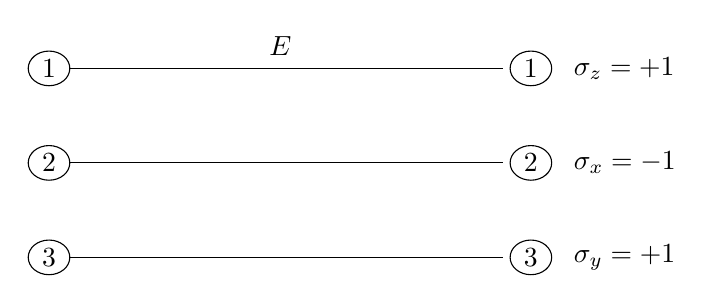
\begin{tikzpicture}[x=1.2cm,y=1cm]
\draw (0,0) circle (0.22) node {1};
\draw (0,-1.2) circle (0.22) node {2};
\draw (0,-2.4) circle (0.22) node {3};

\draw (0.22,0) -- (4.8,0);
\draw (0.22,-1.2) -- (4.8,-1.2);
\draw (0.22,-2.4) -- (4.8,-2.4);

\node at (2.45,0.28) {$E$};

\draw (5.1,0) circle (0.22) node {1};
\draw (5.1,-1.2) circle (0.22) node {2};
\draw (5.1,-2.4) circle (0.22) node {3};

\node[anchor=west] at (5.45,0) {$\sigma_z=+1$};
\node[anchor=west] at (5.45,-1.2) {$\sigma_x=-1$};
\node[anchor=west] at (5.45,-2.4) {$\sigma_y=+1$};
\end{tikzpicture}
\end{figure}

If Bob later sends those outcomes in an ordinary classical message, then Alice can choose to measure along the corresponding axes and will find the opposite result in each case. But the update happens only when the message reaches her.

\subsection{Question \& Answer}

If Bob measures first, when does Alice's density matrix actually change?

As far as Alice is concerned, it changes when Alice receives information that Bob's result has been obtained. Before that, her local state assignment remains the one she had before: a density matrix encoding the probabilities available to her locally. After the telegram arrives, she rationally updates that state assignment. This is not a physical influence traveling faster than light; it is an update of knowledge after ordinary communication.

The second question is Bell's question. If no signals go faster than light, what is the real content of the famous nonlocality discussion? Here the lecture adopts a computer-science game. A single classical computer can simulate a single spin. It stores amplitudes
\begin{equation}
|\psi\rangle=\alpha_u|u\rangle+\alpha_d|d\rangle,
\qquad
|\alpha_u|^2+|\alpha_d|^2=1,
\end{equation}
uses them to compute probabilities, feeds those probabilities into a random number generator, and then updates the stored state after a measurement. As a simulation of one spin, this works.

The trouble begins when we try to simulate an entangled pair with two separated classical computers, one holding Alice's information and one holding Bob's. If the state is a product state, no problem: each side may be simulated independently. But once the pair is entangled, Bell's theorem says that the separated classical machines cannot reproduce the quantum statistics unless there is hidden continuing communication between them. Synchronizing them in advance is not enough. They must keep talking.

This is the sense in which Bell forces a kind of nonclassicality. Not that Bob can use entanglement to signal to Alice instantaneously; quantum mechanics forbids that. Rather, a classically separated description with purely local hidden bookkeeping is not enough to reproduce entangled correlations. One may say that the classical simulation needs hidden wires. Or one may say, as Susskind prefers, that one gets into trouble only by insisting on forcing a quantum phenomenon into a classical picture that is too small for it.

There is an ensemble-level operational lesson at the end. Bob by himself cannot detect entanglement from a single trial. But if he is given many identically prepared copies, he can search for a direction in which his spin is definite. If the state were a product state, some axis would eventually reveal stable repeated results. If the state is entangled as in the singlet, no axis does so; every direction remains locally random. That is the local signature of having only a reduced density matrix and not a pure local wave function.

\section{Summary}

The lecture's line of thought is remarkably tight. First, entanglement is not the fact that a composite system has a state, but the fact that its state need not factorize. Second, wave functions make this precise by turning states into coefficients in a basis. Third, product states imply factorized expectation values and zero correlation. Fourth, the singlet shows the opposite extreme: locally nothing definite, jointly everything fixed that can be fixed. Fifth, the reduced density matrix is the right local object, and its eigenvalues diagnose entanglement. Sixth, measurement is itself an entangling process. Finally, none of this permits superluminal signaling, even though Bell tells us that entangled quantum systems cannot be reproduced by genuinely separated classical simulations without hidden continuing communication.

The oddity remains where Susskind wants it to remain: one may know as much as quantum mechanics allows about a whole system and still know nothing definite about its parts. The mathematics is perfectly sharp. The discomfort, if one feels it, comes afterward.